\section{名前はまだない}
吾輩は猫である.名前はまだない.

どこで生まれたかとんと見当がつかぬ.
何でも薄暗いじめじめした所でニャーニャー泣いていた事だけは記憶している.
吾輩はここで始めて人間というものを見た.
しかもあとで聞くとそれは書生という人間中で一番獰悪な種族であったそうだ.
この書生というのはときどき我々を捕えて煮て食うという話である.
しかしその当時は、何という考もなかったから,別段恐ろしいとも思わなかった.
ただ彼の掌に載せられてスーと持ち上げられた時何だかフワフワした感じがあった
ばかりである.

\begin{figure}
    \centering
    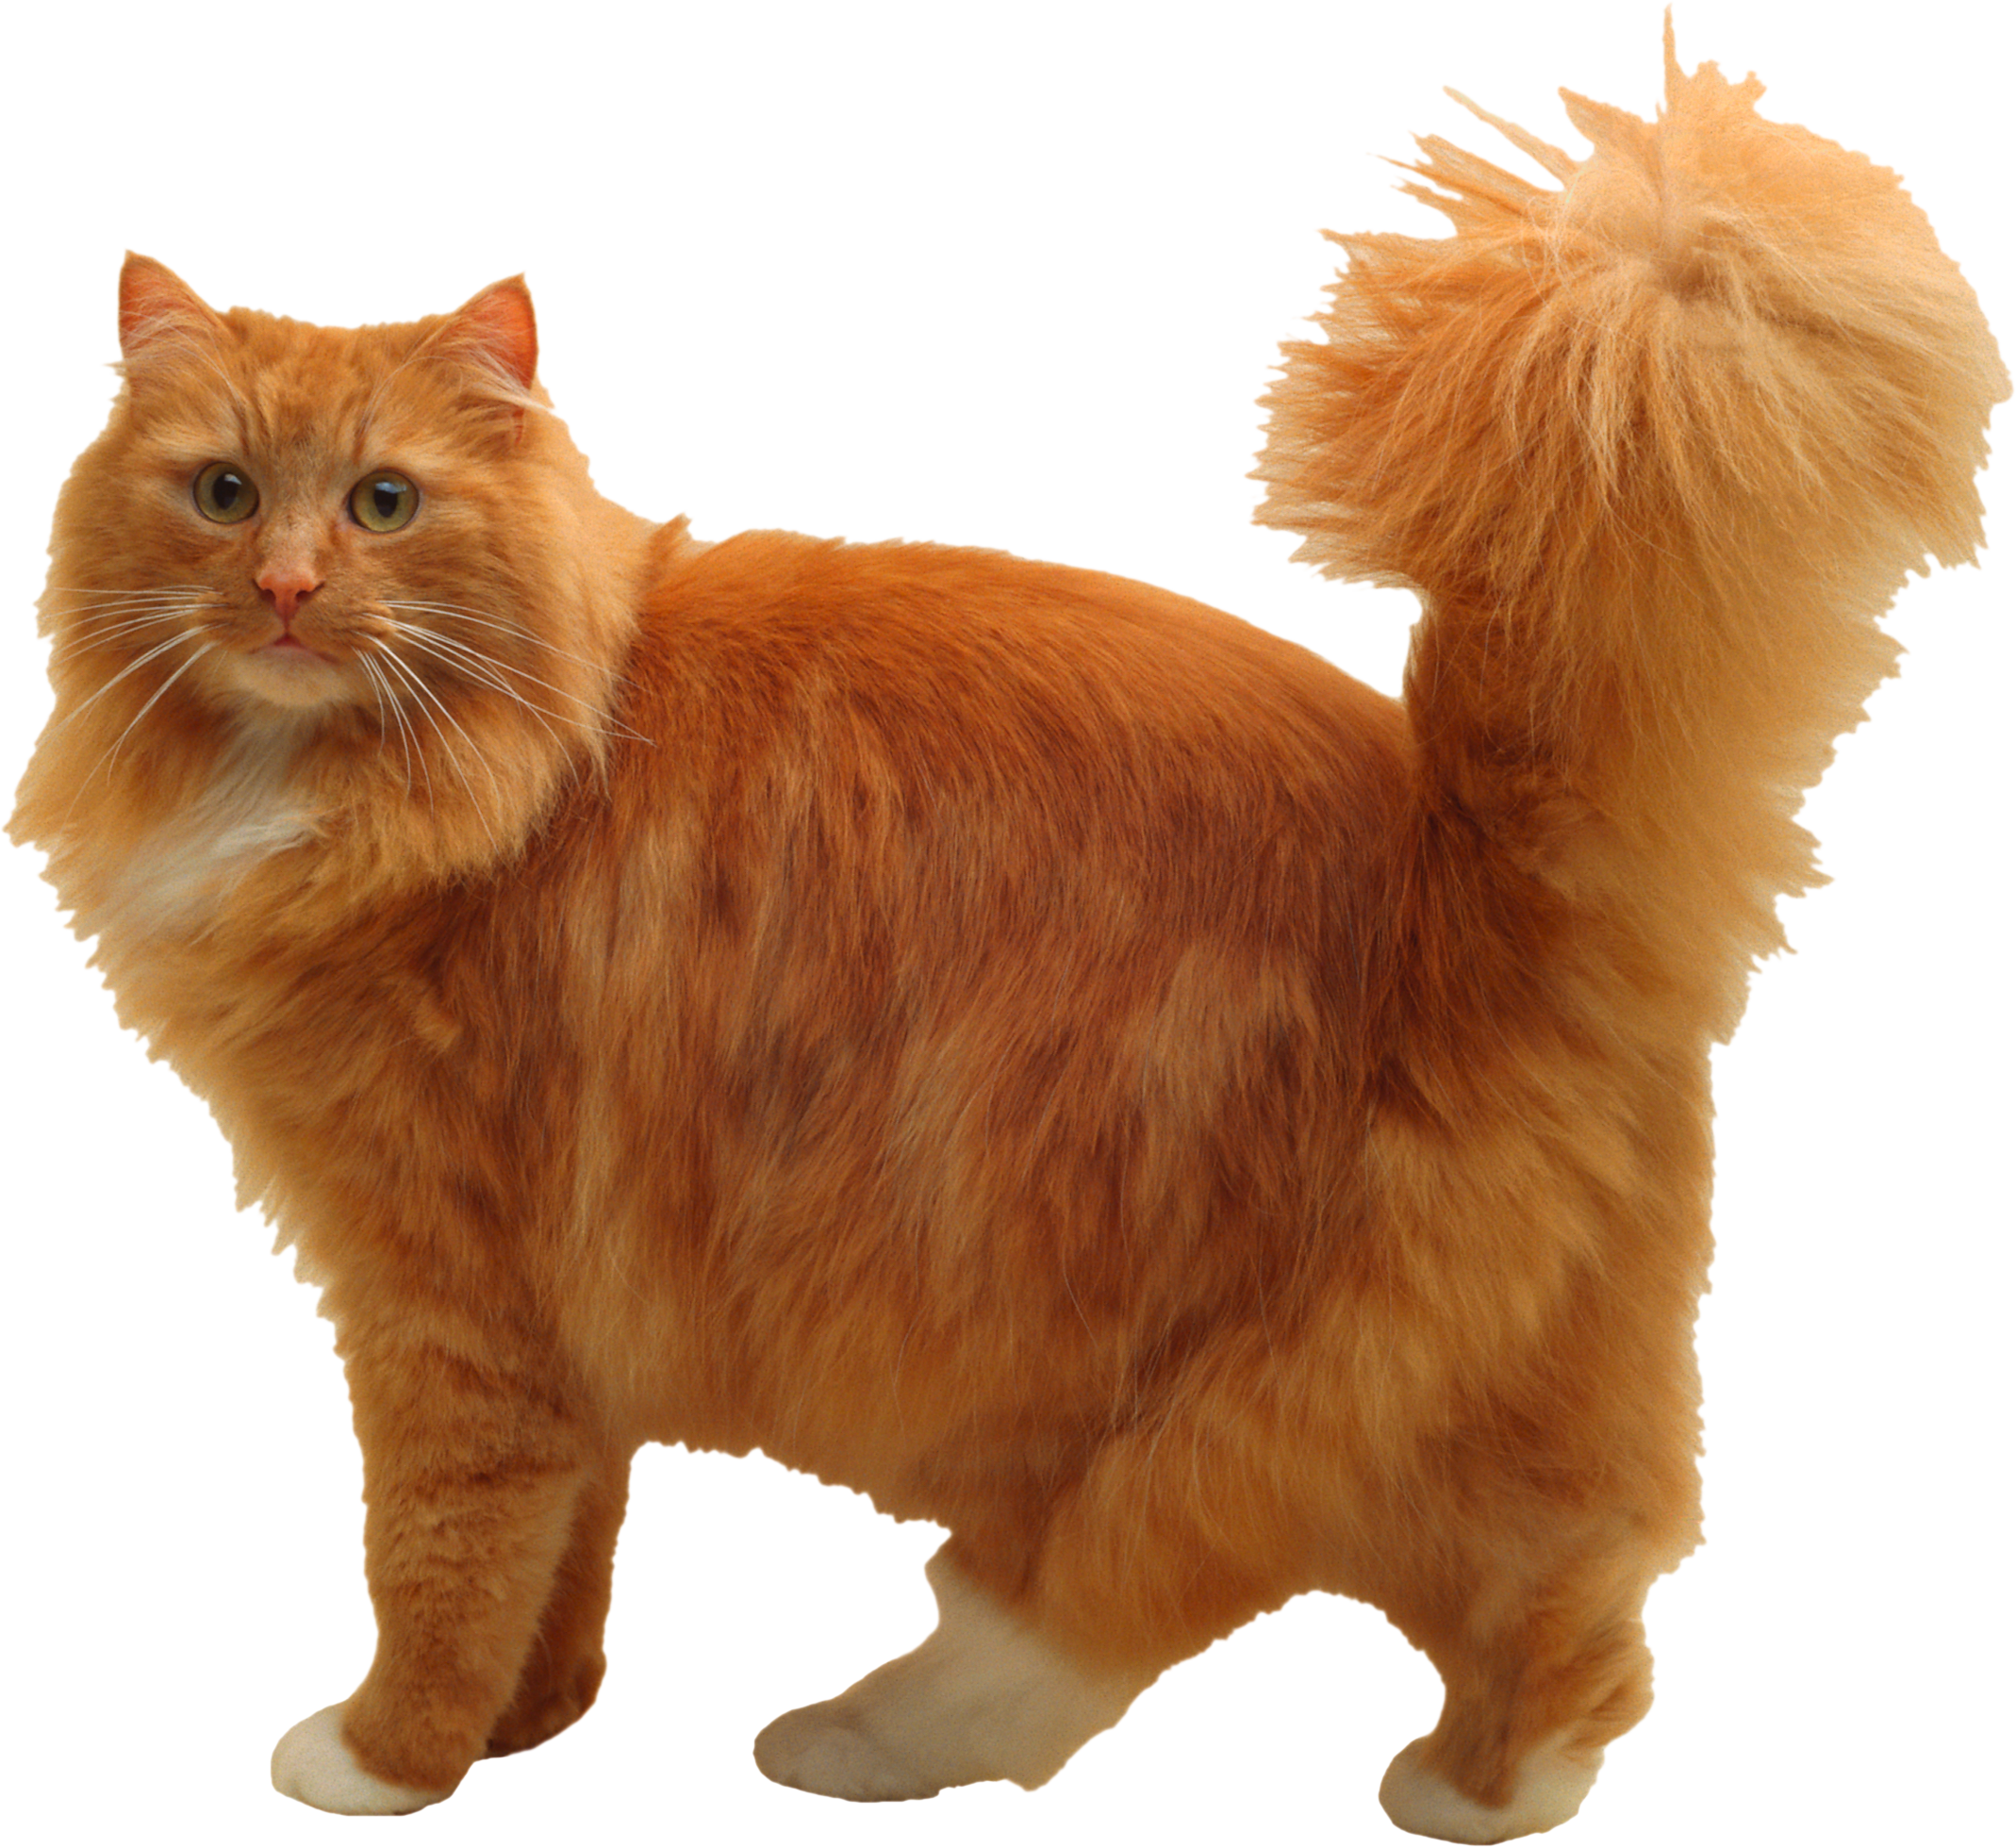
\includegraphics[scale=0.4]{image/cat_1.png}
    \caption{猫の画像 \cite{Freecatp65:online}}
    \label{fig:cat}
\end{figure}